\chapter{Inference as Optimization: An Region-based Energy Method}
\label{chapter4}
In the previous chapter, we explained an iterative message passing algorithm and discussed the connection with mean field, belief propagation, and tree-reweighted belief propagation algorithms. These methods fellow different message passing rules (fixed-point iterations) that are manually developed. The manual efforts in implementation for a practical inference problem include both the message-passing rule definition and also message update schedule, both of which make a significant difference in the performance of approximate inference. However, on our way towards automated inference methods, we intend to reduce the manual efforts without degenerating their performance. In this chapter, we would discuss one promising way to realize this target. The principle idea is to do inference as solving an optimization problem, i.e. inference as optimization.

In fact, we have touched this topic in Section~\ref{chpt2:sec:variational-inference}, where we were trying to interpret what message passing updates of mean field and belief propagation are actually doing. It turns out that the message passing rules are fixed-point iterations as solutions to optimization problems. Therefore mean field and belief propagation get the intuition of minimization of variational free energy. Take the most widely used belief propagation method as an example, since the message passing rule can be obtained from the minimization of Bethe free energy cost, we may just as well solve the optimization problem by other optimization techniques such as gradient descent. But an early attempt on this track showed that it might suffer from the stability for peaky potential functions compared to iterative message passing method \cite{welling2001belief}.


Another limitation lies in the Bethe approximation itself. When representing Bethe approximation in a factor graph (not necessary to be the pairwise case), a factor node associated with a potential function is related with more than one random variable, while a variable node is associated with one random variable. When beliefs are propagated on the graph, only a univariate marginal distribution (associated with a variable node) can be propagated from one neighboring factor to another neighboring factor of the variable node. The interactions between multiple variables can not be directly propagated as messages in the graph. This limitation actually affects the performance of Bethe approximation in general graphs, especially the loopy graphs.

In this chapter, we seek to use larger clusters in a graphical representation to overcome the above-mentioned limitation. Along with that, we would bring the concept of inference as optimization into the alternative representation.




\begin{figure}[!t]
  \centering
  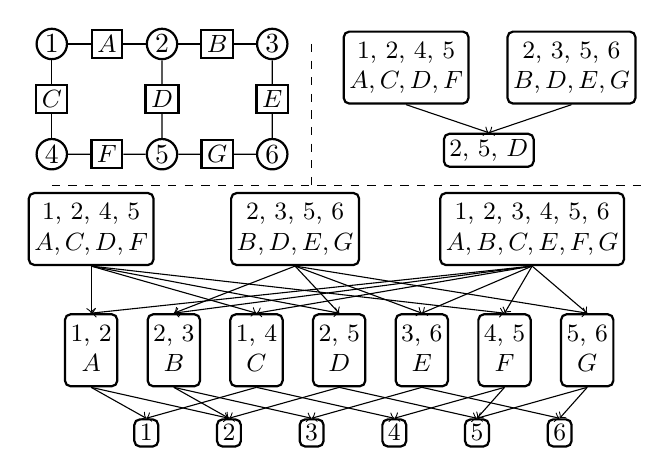
\begin{tikzpicture}
    \begin{scope}[scale=0.7]

      \tikzstyle{cnode} = [thick, draw=black, circle, inner sep = 1pt,  align=center]
      \tikzstyle{nnode} = [thick, rectangle, rounded corners = 0pt,draw,inner sep = 2pt]
      \node[cnode] (x1) at (0,0) {1};
      \node[cnode] (x2) at (2,0) {2};
      \node[cnode] (x3) at (4,0) {3};

      \node[cnode] (x4) at (0,-2) {4};
      \node[cnode] (x5) at (2,-2) {5};
      \node[cnode] (x6) at (4,-2) {6};

      \node[nnode] (fa) at (1,0) {\small$A$};
      \node[nnode] (fb) at (3,0) {\small$B$};

      \node[nnode] (fc) at (0,-1) {\small$C$};
      \node[nnode] (fd) at (2,-1) {\small$D$};
      \node[nnode] (fe) at (4,-1) {\small$E$};
      
      \node[nnode] (ff) at (1,-2) {\small$F$};
      \node[nnode] (fg) at (3,-2) {\small$G$};


      \draw[-] (x1) -- (fa);
      \draw[-] (x1) -- (fc);

      \draw[-] (x2) -- (fa);
      \draw[-] (x2) -- (fb);
      \draw[-] (x2) -- (fd);

      \draw[-] (x3) -- (fb);
      \draw[-] (x3) -- (fe);

      \draw[-] (x4) -- (fc);
      \draw[-] (x4) -- (ff);

      \draw[-] (x5) -- (fd);
      \draw[-] (x5) -- (ff);
      \draw[-] (x5) -- (fg);

      \draw[-] (x6) -- (fe);
      \draw[-] (x6) -- (fg);

    \end{scope}
    \draw[dashed] (0, -1.8) -- (7.5, -1.8) (3.3, 0) -- (3.3, -1.8);
    
    \begin{scope}[xshift=4.5cm, yshift=-0.3cm,scale=0.7]
      \tikzstyle{rnode} = [thick, rectangle, rounded corners = 2pt,minimum size = 0.0cm,draw,inner sep = 2pt]
      \node[rnode] (r01) at (0,0) {\small \begin{tabular}[x]{@{}c@{}}1, 2, 4, 5 \\ $A,C,D,F$ \end{tabular}};
      \node[rnode] (r02) at (3,0) {\small \begin{tabular}[x]{@{}c@{}}2, 3, 5, 6\\ $B,D,E,G$ \end{tabular}};
      \node[rnode] (r11) at (1.5, -1.5) {\small 2, 5, $D$};

      \draw[->] (r01.south) -- (r11.north);
      \draw[->] (r02.south) -- (r11.north);

    \end{scope}

    \begin{scope}[xshift=0.5cm, yshift=-2.35cm,scale=0.7]
      \tikzstyle{rnode} = [thick, rectangle, rounded corners = 2pt,minimum size = 0.0cm,draw,inner sep = 2pt]
      \node[rnode] (r01) at (0,0) {\small\begin{tabular}[x]{@{}c@{}}1, 2, 4, 5 \\ $A,C,D,F$ \end{tabular}};
      \node[rnode] (r02) at (3.7,0) {\small\begin{tabular}[x]{@{}c@{}}2, 3, 5, 6\\ $B,D,E,G$ \end{tabular}};
      \node[rnode] (r03) at (8,0) {\small\begin{tabular}[x]{@{}c@{}}1, 2, 3, 4, 5, 6\\ $A,B,C,E,F,G$ \end{tabular}};
      \begin{scope}[yshift=-0.2cm]
        \node[rnode] (r11) at (0, -2.0) {\small\begin{tabular}[x]{@{}c@{}}1, 2\\ $A$ \end{tabular}};
        \node[rnode] (r12) at (1.5, -2.0) {\small\begin{tabular}[x]{@{}c@{}}2, 3\\ $B$ \end{tabular}};
        \node[rnode] (r13) at (3, -2.0) {\small\begin{tabular}[x]{@{}c@{}}1, 4\\ $C$ \end{tabular}};
        \node[rnode] (r14) at (4.5, -2.0) {\small\begin{tabular}[x]{@{}c@{}}2, 5\\ $D$ \end{tabular}};
        \node[rnode] (r15) at (6, -2.0) {\small\begin{tabular}[x]{@{}c@{}}3, 6\\ $E$ \end{tabular}};
        \node[rnode] (r16) at (7.5, -2.0) {\small\begin{tabular}[x]{@{}c@{}}4, 5\\ $F$ \end{tabular}};
        \node[rnode] (r17) at (9, -2.0) {\small\begin{tabular}[x]{@{}c@{}}5, 6\\ $G$ \end{tabular}};

        \begin{scope}[yshift=0.5cm]
          \node[rnode] (r21) at (1, -4) {\small 1};
          \node[rnode] (r22) at (2.5, -4) {\small 2};
          \node[rnode] (r23) at (4, -4) {\small 3};
          \node[rnode] (r24) at (5.5, -4) {\small 4};
          \node[rnode] (r25) at (7, -4) {\small 5};
          \node[rnode] (r26) at (8.5, -4) {\small 6};
        \end{scope}
      \end{scope}
      % edge level0 to level1
      \draw[->] (r01.south) -- (r11.north);
      \draw[->] (r03.south) -- (r11.north);

      \draw[->] (r02.south) -- (r12.north);
      \draw[->] (r03.south) -- (r12.north);

      \draw[->] (r01.south) -- (r13.north);
      \draw[->] (r03.south) -- (r13.north);

      \draw[->] (r01.south) -- (r14.north);
      \draw[->] (r02.south) -- (r14.north);

      \draw[->] (r02.south) -- (r15.north);
      \draw[->] (r03.south) -- (r15.north);

      \draw[->] (r01.south) -- (r16.north);
      \draw[->] (r03.south) -- (r16.north);

      \draw[->] (r02.south) -- (r17.north);
      \draw[->] (r03.south) -- (r17.north);

      % edge level1 to level2
      \draw[->] (r11.south) -- (r21.north);
      \draw[->] (r13.south) -- (r21.north);

      \draw[->] (r11.south) -- (r22.north);
      \draw[->] (r12.south) -- (r22.north);
      \draw[->] (r14.south) -- (r22.north);


      \draw[->] (r12.south) -- (r23.north);
      \draw[->] (r15.south) -- (r23.north);

      \draw[->] (r13.south) -- (r24.north);
      \draw[->] (r16.south) -- (r24.north);

      \draw[->] (r14.south) -- (r25.north);
      \draw[->] (r16.south) -- (r25.north);
      \draw[->] (r17.south) -- (r25.north);

      \draw[->] (r15.south) -- (r26.north);
      \draw[->] (r17.south) -- (r26.north);
    \end{scope}
  \end{tikzpicture}
  \caption{Illustration of a factor graph for 2-by-3 grid (top left, variable nodes are indexed by number and factor nodes by letters), and two alternative regions graphs (two levels for the top right one and three levels for bottom one) constructed from the factor graph.}
  \label{fig:factor-region-graphs}
\end{figure}

\section{Region Graph and Generalized Belief Propagation}

In a MRF, the underlining probability distribution of its $N$-dimensional random vector $\bm{x}=(x_1, x_2, \cdots, x_N)$ can be written as
\begin{equation}\label{eq:joint-px}
  p(\bm{x}; \bm{\theta}) = \frac{1}{Z(\bm{\theta})} \prod_{a \in \Ff} \phi_{a}(\bm{x}_{a}; \bm{\theta}_a),
\end{equation}
where potential functions' index set is instantiated as $\Ff = \left\{ A, B, \cdots, M \right\}$. Here we explicitly denote that potential $\phi_a$ has its own parameter $\bm{\theta}_a$, and $\bm{\theta} = \{\bm{\theta}_a, a\in \Ff\}$. For notation simplicity, we define that each variable has $K$ states, i.e. $x_i \in \Xx_i$ with $|\Xx_i|=K$, where $|\cdot|$ denotes the cardinality.

We have discussed that loopy BP as a message-passing algorithm operates on factor graphs (as the top-left example in Figure~\ref{fig:factor-region-graphs}) in Section~\ref{chpt2:sec:variational-inference}. We then can compute the marginal distributions or most likely $\bm{x}$ of \eqref{eq:joint-px} with collection of messages after their propagation under rule \eqref{chpt2:eq:loopy-bp} or its variants discussed in Chapter~\ref{chapter3}. The fundamental limitation of methods in this family that a message over a single variable is communicated instead of over pairs of variables or multiple variables (as stated at the beginning of this chapter). This issue can be relieved by using a hyper-graph or cluster graph where a node is associated with multiple variables. Region graph is such kind of graphs, which was proposed by \cite{yedida2005constucting, DBLP:journals/corr/abs-1207-4158} to assist scheduling messages for generalized belief propagation (GBP). For the illustration purpose, two alternative region graphs constructed from the same factor graph are shown in Figure~\ref{fig:factor-region-graphs}.

Before giving definition of region graph, we need to define \textit{region} first, which is on the basis of factor graph $\Gg_{\Ff}(\Vv \cup \Ff, \Ee_{\Ff})$ (Definition~\ref{chpt2:def:factor-graph}).
\begin{definition}
  A \textit{region} $R$ is a set $V_R$ of variables nodes and a set $A_R$ of factor nodes, such that if a factor node $a$ belong to $A_R$, all the variables nodes neighboring $a$ are in $V_R$.
\end{definition}
A region in a region graph acts a node and there are directed edges between regions which are defined according to specific rules. Formally, a region graph is defined as bellow.
\begin{definition}\label{def:region-graph}
  A \textit{region graph} is  a directed graph $\Gg_R(\Rr, \Ee)$, where each vertex $R \in \Rr$ is defined as the joint set of variable and factor nodes in this region, i.e. $R = \left\{ i \in V_R, a \in A_R | i \in \Vv, a \in \Ff \right\}$. Each edge $e \in \Ee$ in $\Gg_R$ is directed from $R_p$ to $R_c$ such that $R_c \subset R_p$. 
\end{definition}


We define some notations before going further. Since $\Gg_R$ is a hierarchical directed graph, $\Rr_l$ denotes regions in level $l$, and 
$R^{[l]}_i\in \Rr_l$ denotes $R^{[l]}_i$ is the $i$-th region node in level $l$. This means $\Rr_0$ is a set of the top root regions that have no parents, i.e. the level $0$ regions. Also, $R^{[l]}$ means it can be any node in $\Rr_l$ and $R$ denotes a region node when it is not clear or doesn't matter which level it locates. Lastly, due to a region may be associated with both variable and factor, we denote the scope of $R$ by  $\bm{x}_R = \left\{ x_i| i \in R \right\}$.

\begin{example}
  Take the top-right region graph in Figure~\ref{fig:factor-region-graphs} as an example. There are total two layers in the region graph, i.e., $\Rr_0$ and $\Rr_1$. We have $\Rr_0 = \left\{ R_1^{[0]}, R_2^{[0]} \right\}$ where $R_1^{[0]} = \left\{ 1, 2, 4, 5, A, C, D, F \right\}$ and $R_2^{[0]} = \left\{ 2, 3, 5, 6, B, D, E, G \right\}$. As for $\Rr_1$, there is only one region in it and it is $R_1^{[1]} = \left\{ 2, 5, D \right\}$. There are two directed edges, i.e., $\left( R_1^{[0]}, R_1^{[1]} \right)$ and $\left( R_2^{[0]}, R_1^{[1]} \right)$.
\end{example}

GBP operates on region graph $\Gg_R(\Rr,\Ee)$. A message is always sent from a parent region $P$ to a child region $R$, i.e. the directed edge $(P, R)\in \Ee$. Let us define the factors in region $R$ as $A_R = \left\{ a | a \in R \right\}$. $\Pp(R)$ denotes the set of parent regions of $R$. The descendants of $R$ is denoted by $\Dd(R)$ (excluding $R$). The descendants of $R$ including $R$ is denoted by $\hat{\Dd}(R) = \Dd(R) \cup R$. The message update rule from the parent region $P$ to the child region $R$ is
\begin{align}
  m_{P\rightarrow R} \propto \frac{\sum_{\bm{x}_P\backslash
  \bm{x}_R}\prod_{a\in A_P\backslash A_R}\phi_a(\bm{x}_a)\prod_{(I,J)
  \in \Nn(P, R)}m_{I\rightarrow J}(\bm{x}_J)}{\prod_{(I,J)
  \in \Hh(P, R)}m_{I\rightarrow J}(\bm{x}_J)},
\end{align}
where
\begin{align}
  \Nn(P, R) &= \left\{ (I,J)\in \Ee | J \in \hat{\Dd}(P) \backslash \hat{\Dd}(R), I \not\in \hat{\Dd}(P)\right\},\nonumber \\
  \Hh(P, R) &= \left\{ (I,J) \in \Ee | J \in \hat{\Dd}(R), I \in \hat{\Dd}(P) \backslash \hat{\Dd}(R) \right\}.
\end{align}
By comparing the GBP with previously discussed mean field, loopy BP and $\alpha$-BP in Chapter~\ref{chapter2} and \ref{chapter3}, it can be seen that both the message update of GBP is more complex. The ordering or sequence of GBP message updates in a region graph also affects it performance (e.g., see \cite{yedida2005constucting}). After message passing phase, the belief for each region $R$, i.e., the approximation to marginal $p(\bm{x}_{R})$, is computed as
\begin{align}
  b_R(\bm{x}_R) \propto \prod_{a\in A_R} \phi_a(\bm{x}_a) \prod_{P\in
  \Pp(R)} m_{P\rightarrow R}(\bm{x}_R) \prod_{D\in \Dd(R)} \prod_{P^{\prime} \in \Pp(D) \backslash \hat{\Dd}(R)} m_{P^{\prime}\rightarrow D}(\bm{x}_D).
\end{align}





\section{Region-based Free Energy}
Recall that BP corresponds to the minimization of Bethe free energy (Section~\ref{chpt2:sec:variational-inference}), it is interesting to note that GBP also corresponding to a free energy defined over region graphs, i.e., \textit{region-based free energy}.
For each region $R$ in a region graph, it has its own region energy, defined as follows.
\begin{definition}
  Given a region $R$ in $\Gg$ and $\bm{\theta}_R=\{\bm{\theta}_a, a\in A_R\}$, the region energy is defined to be
  \begin{equation}
    E_R(\bm{x}_R; \bm{\theta}_R) = - \sum_{a\in A_R} \ln{\phi_a(\bm{x}_a; \bm{\theta}_a)}.
  \end{equation}
\end{definition}
The region-based free energy over a region graph $\Gg_R$ is defined over the region energies and also the region beliefs. Formally, the region-based free energy is defined as follows.
\begin{definition}\label{def:region-free-energy}
  For any region graph $\Gg_R$, the region-based free energy is defined as
  \begin{equation}\label{eq:def-region-free-energy}
    F_R(\Bb; \bm{\theta}) = \hspace{-0.15cm}\sum_{R\in \Rr} \hspace{-0.1cm}c_R\hspace{-0.1cm} \sum_{\bm{x}_R}b_R(\bm{x}_R) (E_R(\bm{x}_R; \bm{\theta}_R) + \ln{b_R}(\bm{x}_R)),
  \end{equation}
  where $b_R(\bm{x}_R)$ is the belief to region $R$, $\Bb$ is the set of region beliefs $\Bb = \left\{ b_R| R \in \Rr \right\}$, and integer $c_R \in \NN$ is the counting number for region $R$.
\end{definition}

Region-based free energy is a more generalized free energy than the variational free energy discussed in Section~\ref{chpt2:sec:variational-inference}. For instance, Bethe free energy, corresponding loopy BP, can be viewed as a special case of region-based free energy.

\subsection{Recover Bethe Free Energy from Region-based Free Energy}
\label{apdix:sec:get-bethe-from-region-energy}
If we define two types of regions (large regions and small
regions) directly from a factor graph $\Gg_F(\Vv \cup \Ff, \Ee_F)$, which is two-level region graph with large regions locate in root level (level 0) and small regions locate in the level 1, we have
\begin{align}
  \Rr_{L} &= \left\{ a, \bm{x}_a| a\in \Ff \right\}, \nonumber \\
  \Rr_{S} &= \left\{ i | i \in \Vv \right\}.
\end{align}
The edges of the original factor graph $\Gg_F$ are preserved in the constructed region graph with adding directions from a factor node to its neighboring variable nodes. For the large regions, we set counting number $c_{R,a}=1$, and for small regions each node $i$, set counting number $c_{R,i}=1-|\mathrm{ne}_i|$. Then we can recover the Bethe free energy from region-based free energy defined in 
\eqref{eq:def-region-free-energy}. To be specific, for
large regions,
\begin{align}\label{apdix:eq:large-region}
  F_{R,L} &=\sum_{R\in \Rr_{L}} c_{R,a}
            \sum_{\bm{x}_R}b_R(\bm{x}_R) (E_R(\bm{x}_R;\bm{\theta}_R) + \ln{b_R}(\bm{x}_R))
            \nonumber \\
          & =\sum_{a\in \Ff} \sum_{\bm{x}_a} b_a(\bm{x}_a)\ln{\frac{b_a(\bm{x}_a)}{\phi_a(\bm{x}_a; \bm{\theta}_a)}}.
\end{align}
And for the small regions, the free energy can be similarly obtained as
\begin{equation}\label{apdix:eq:small-region}
  F_{R,S}  =  \sum_{i=1}^{N} (1- |\mathrm{ne}_i|) \sum_{x_i} b_i(x_i) \ln{b_i(x_i)}.
\end{equation}
Putting \eqref{apdix:eq:large-region} and \eqref{apdix:eq:small-region} together recovers the Bethe free energy \eqref{chpt2:bethe-free-energy}.






\section{Region-based Energy Neural Network}

\begin{figure}[!t]
  \centering
  \begin{tikzpicture}
    
    \tikzstyle{enode} = [thick, draw=black, ellipse, inner sep = 2pt,  align=center]
    \tikzstyle{cnode} = [thick, draw=black, circle, inner sep = 0.0pt,  align=center]
    \tikzstyle{nnode} = [thick, rectangle, rounded corners = 0pt,draw,inner sep = 2pt]
    \begin{scope}[xshift=-1cm, yshift=-1.3cm, scale=0.6]
      \node[enode, rotate=90] (em) at (-2.5,0) {Embedings};
      \node[enode, rotate=90] (nn) {Neural Network};
    \end{scope}
    
    % level0 regions
    \begin{scope}[scale=0.6]
      \node[cnode] (r01) at (1, 0) {\tiny$R_1^{[0]}$};
      \node[cnode] (r02) at (1, -1) {\tiny$R_2^{[0]}$};
      \node[cnode] (r03) at (1, -2) {\tiny$R_3^{[0]}$};
      \node[cnode] (r04) at (1, -3) {\tiny$R_4^{[0]}$};
      \node[cnode] (r05) at (1, -4) {\tiny$R_5^{[0]}$};
      \node[label=below:$\Rr_0$, draw,rounded corners = 2pt, inner sep=1mm, fit=(r01) (r05)] {};
    \end{scope}

    \draw[->] (nn.351.9) |- (r01);
    \draw[->] (nn.340) |- (r02);
    \draw[->] (nn.295) |- (r03);
    \draw[->] (nn.210) |- (r04);
    \draw[->] (nn.191) |- (r05);

    \draw[->] (em) -- (nn);


    % level 1 regions
    \begin{scope}[xshift=1.5cm, yshift=-0.2cm, scale=0.6]
      \node[cnode] (r11) at (1, 0) {\tiny$R_1^{[1]}$};
      \node[cnode] (r12) at (1, -1) {\tiny$R_2^{[1]}$};
      \node[cnode] (r13) at (1, -2) {\tiny$R_3^{[1]}$};
      \node[cnode] (r14) at (1, -3) {\tiny$R_4^{[1]}$};
      \node[label=below:$\Rr_1$, draw, rounded corners = 2pt, inner sep=1mm, fit=(r11) (r14)] {};
    \end{scope}

    
    
    % level 1 regions
    \begin{scope}[xshift=3cm, yshift=-0.2cm, scale=0.6]
      \node[cnode] (r21) at (1, 0) {\tiny$R_1^{[2]}$};
      \node[cnode] (r22) at (1, -1) {\tiny$R_2^{[2]}$};
      \node[cnode] (r23) at (1, -2) {\tiny$R_3^{[2]}$};
      \node[cnode] (r24) at (1, -3) {\tiny$R_4^{[2]}$};
      \node[label=below:$\Rr_2$, draw, rounded corners = 2pt, inner sep=1mm, fit=(r21) (r24)] {};
    \end{scope}

    \draw[->] (r01) -- (r11);
    \draw[->] (r03) -- (r11);

    \draw[->] (r02) -- (r12);
    \draw[->] (r04) -- (r12);
    \draw[->] (r05) -- (r12);

    \draw[->] (r01) -- (r13);
    \draw[->] (r04) -- (r13);

    \draw[->] (r03) -- (r14);
    \draw[->] (r05) -- (r14);


    \draw[->] (r11) -- (r21);
    \draw[->] (r14) -- (r21);

    \draw[->] (r11) -- (r22);
    \draw[->] (r13) -- (r22);

    \draw[->] (r12) -- (r23);
    \draw[->] (r14) -- (r23);

    \draw[->] (r12) -- (r24);
    \draw[->] (r13) -- (r24);

    
    
  \end{tikzpicture}
  
  \caption{Illustration of a RENN with three levels of regions ($\Rr_0$, $\Rr_1$, $\Rr_2$).}
  \label{fig:renn-illustration}
  
\end{figure}


In this section, we explain how the proposed region-based energy neural network (RENN) works.
We are interested in finding marginal probabilities such as $p(\bm{x}_R)$. A region belief $b_R(\bm{x}_R)$ an approximation to $p(\bm{x}_R)$.
Instead of propagating messages as GBP, or directly optimize w.r.t. variables ${b_R(\bm{x}_R)}$ of interests, we use the reparameterization technique that is also used by recent works \cite{DBLP:journals/corr/KingmaW13, srikumar-etal-2012-amortizing, NIPS2019_9687, akbayrak2019reparameterization}, to model the values of interests to be the output of a neural network. We then optimize w.r.t. the parameters of the neural network. This technique is called amortizing.

Note that in RENN, the neural network only needs to directly model beliefs on root regions $\Rr_0$. The beliefs of non-root regions $\Rr_l,~l>0$ could be obtained from root region beliefs according to the structure of the region graph. This can reduce the number of neural network parameters compared to directly modeling the beliefs of all regions.

\subsection{Inference by RENN}
\label{sec:infer-renn}

For a root region $R^{[0]}\in \Rr_0$, our RENN has a corresponding vector representing its score $\bm{f}(\Gg_R, R^{[0]}; \bm{\omega}) \in \RR^{|{\bm{x}_{R^{[0]}}}| \times K}$, where $\bm{\omega}$ is the parameter of mapping $\bm{f}$ that is modeled by a neural network. We define the predicted belief on the root region node $R^{[0]}$ as
\begin{equation}
  b_{R^{[0]}}(\bm{x}_{R^{[0]}}; \bm{\omega}) := \sigma(\bm{f}(\Gg_R, R^{[0]}; \bm{\omega})), \forall~ {R^{[0]}} \in \Rr,
\end{equation}
where $\sigma(\cdot)$ is the softmax function.

The representation mapping $\bm{f}$ followed by the softmax function in a RENN only needs to directly output the beliefs on root regions $\Rr_0$.
For the rest regions $\left\{R \in \Rr \backslash \Rr_0 \right\}$ that are not root regions in the region graph, where $\backslash$ denotes the set exclusion, the RENN computes the belief as
\begin{equation}\label{eq:l-level-beliefs}
  b_{R^{[l]}}(\bm{x}_{R^{[l]}}; \bm{\omega}) = \frac{1}{|\Pp(R^{[l]})|} \sum_{R_p\in  \Pp(R^{[l]})}\sum_{\bm{x}_{R_p}\backslash \bm{x}_{R^{[l]}}} b_{R_p}(\bm{x}_{R_p}; \bm{\omega}),
\end{equation}
where $\Pp(R^{[l]})$ is the set of parent regions of $R^{[l]}$ in region graph $\Gg_R$. The non-root region belief of RENN defined in this way comes with the intuition of typical iterative belief propagation methods. In BP and its variants, messages are passed to a variable node to reduce the mismatch of beliefs w.r.t. the variable node, which are sent from this node's neighbors in a factor graph. The message passing iteration of BP or its variants stops when this kind of mismatch w.r.t. every variable node is eliminated in the factor graph, i.e., converged.

In RENN, we directly cast the mismatch between a non-root region belief $b_{R^{[l]}}(\bm{x}_{R^{[l]}}; \bm{\omega})$ and the marginalization from its parent region $\sum_{\bm{x}_{R_p}\backslash \bm{x}_R^{[l]}}b_{R_p}(\bm{x}_{R_p}; \bm{\omega})$ as a penalty in the cost function. As the mismatch penalty is close to zero, the non-root region belief gets close to marginalization calculated from its parent regions. Matching a region's belief with marginalization from its parent regions' beliefs is termed as region belief consistency in region graph. That is to say, apart from averaging effect from definition itself \eqref{eq:l-level-beliefs}, a hard-penalty is enforced straightforwardly in our cost.

Different from GBP that minimizes region-based free energy by iterative message-passing, RENN minimizes the region-based free energy by optimizing w.r.t. the neural network parameter $\bm{\omega}$.
Considering the region belief consistency, we summarize the cost function of RENN to include both the region-based free energy and mismatch penalty on non-root regions. This gives the optimization problem:
\begin{equation}\label{eq:infer-F-all-belief}
  \umin{\bm{\omega}}{F_R(\Bb;\bm{\theta}) + \lambda \sum_{R\in \Rr \backslash \Rr_0} \sum_{R_p \in \Pp(R)} d( b_R, \sum_{\bm{x}_{R_p}\backslash \bm{x}_{R}} b_{R_p}(\bm{x}_{R_p}; \bm{\omega}))},
\end{equation}
where $d(\cdot, \cdot)$ is distance metric or divergence to measure the mismatch between the beliefs ($L_2$ distance is used in our experiments), $\lambda$ is a positive regulation parameter. In a word, a RENN takes embedding vectors as input and output beliefs directly by minimizing regularized region-based free energy. Embedding vectors are tunable variables (part of paramter $\bm{w}$), and would be explained in Section~\ref{subsec:exp-setting}, although not explicit in the objective function \eqref{eq:infer-F-all-belief}.


\begin{example}
  We demonstrate a toy RENN in this example. As illustrated in Figure~\ref{fig:renn-illustration}, a three-level RENN takes embedding vectors as input and outputs the beliefs on $\Rr_0$ directly. The beliefs in other levels $\{\Rr_1$, $\Rr_2\}$ are computed as in \eqref{eq:l-level-beliefs}. Then the region-based free energy along with the penalty of region belief consistency is minimized w.r.t. $\bm{\omega}$.
\end{example}

\begin{remark}[Region-based Free Energy and the Partition Function]
  We explained in Section~\ref{chpt2:sec:variational-inference} that Bethe free energy is an approximation to the negative log-partition function, i.e., $-\log{Z(\bm{\theta})}$. This relationship between free energy and partition function similarly exists for RENN.
  After the energy minimization phase as stated in \eqref{eq:infer-F-all-belief}, the minimized region-based free energy $F_R(\Bb^{\ast};\bm{\theta})$ is an approximation to the negative log-partition $-\log{Z(\bm{\bm{\theta}})}$, where $\Bb^{\ast} = \left\{b_R(\bm{x}_R;\bm{\omega}^{\ast})| R \in \Rr \right\}$ with $\bm{\omega}^{\ast}$ as the parameter of RENN after the optimization phase.
\end{remark}

\subsection{Region Graph Construction for RENN}
In this section we detail how to construct the region graph $\Gg_R$ for RENN.
Informally, a region graph can be generated by firstly clustering the nodes in a factor graph in any way and then connect the clusters with directed edges as long as the resulted graph should fulfill the Definition~\ref{def:region-graph}. But it does not mean we can rely on an arbitrary region graph to do our inference. Conditions such as \textit{valid} region graph (would be discussed in the following subsection), and \textit{maxent-normality} \cite{yedida2005constucting,welling2005structured} have been proposed for region graphs. But these conditions do not gives rules of how to construct ''good'' region graphs.
Our idea for this issue is to combine the cluster variation method \cite{PhysRev.81.988,morita1991cluster} with \textit{tree-robust} condition \cite{gelfand2012generalized} (that was originally developed to improve accuracy of GBP) for practical region graph construction.

In what follows, we firstly explain the concept of valid region graphs. Then the method of region graph construction for RENN is detailed.

\subsubsection{Determining the Counting Numbers}
\label{subsec:count-number}
In Definition~\ref{def:region-free-energy}, region-based free energy is defined as a function of counting numbers $\left\{ c_R \right\}$. The counting numbers here are used to balance each region's contribution to the free energy. According to \cite{yedida2005constucting}, the region-base free energy is \text{valid} if the following $1$-balanced conditions holds
\begin{equation}\label{eq:1-ballanced-condition}
  \sum_{R\in\Rr} c_R \delta_{R}(i)  = 1, \forall~ \mathrm{node}~ i~~ \mathrm{in} ~~\Gg_F,
\end{equation}
where $\delta_{R}(i)$ is the indicator function, equal to $1$ if and only if node $i$ defined in factor graph $\Gg_F$ falls in the region $R$ of the region graph $\Gg_R$ and equal to $0$ otherwise. Note that node $i$ can be either a variable or factor node here. It can be seen that each node would be counted exactly once if the condition \eqref{eq:1-ballanced-condition} holds.

Given a region graph $\Gg_R$, the counting numbers $\left\{ c_R \right\}$ can be constructed recursively as
\begin{equation}
  c_R = 1 - \sum_{R_i \in \Aa(R)} c_{R_i}, \forall R,
\end{equation}
where $\Aa(R)$ denotes the ancestor set of region node $R$ in $\Gg_R$. This rule means the counting numbers of root regions are always $1$, since they do not have any ancestors.


\subsubsection{Generating Graph by Cluster Variation Method}
\label{sec:cluster-variation-method}
Cluster variation method was introduced by Kikuchi and other physicists \cite{PhysRev.81.988,morita1991cluster}, which started with the intuition of approximating free energy by using larger sets of variable nodes instead of the single-node factorization in mean field approximation.

Cluster variation method starts with the root regions $\Rr_0$. There are two requirements for $\Rr_0$: i) every variable node $i$ of factor graph $\Gg_F$ is included in at least one region $R^{[0]}\in\Rr_0$; ii) there should be no region $R^{[0]}\in \Rr_0$ being a subregion of any other region in $\Rr_0$.
With $\Rr_0$ ready, the other sets of regions are generated hierarchically. To construct level-$1$ regions $\Rr_1$ from $\Rr_0$, we find out all the intersections between regions in $\Rr_0$, but omit any that are subregion of other intersection regions. Then level-$2$ regions $\Rr_2$ can be similarly constructed from $\Rr_1$. Assume there are $L$ such sets, then $\Rr = \Rr_0 \cup \Rr_1 \cup \cdots \cup \Rr_{L-1}$. The construction rule can be formulated as
\begin{align}
  \Rr_l = &\{ R^{[l]}_i := R^{[l-1]}_j \cap R^{[l-1]}_k | R^{[l]}_i \not\subset R^{[l]}_n,~ \forall i \neq n, \nonumber \\
          &R^{[l-1]}_j, R^{[l-1]}_k \in \Rr_{l-1} , j\neq k\}, l=1, 2, \cdots, L-1.
\end{align}

With the hierarchical region sets built, we need to draw the edges. The directed edges are always connected from regions in $\Rr_{l-1}$ to these in $\Rr_{l}$. For one region $R^{[l]}$ in $\Rr_l$, a directed edge is drawn from any superregion of $R^{[l]}$ in $\Rr_l$. This can be represented as
\begin{align}
  \Ee = \{ e := (R^{[l-1]}, R^{[l]}) | R^{[l]} \subset R^{[l-1]}, R^{[l]} \in \Rr_l, R^{[l-1]} \in \Rr_{l-1} , \forall l\}.
\end{align}



\subsubsection{Root Region Construction}
\label{sec:criteria-root-regions}
In Section~\ref{sec:cluster-variation-method}, we detailed the region graph construction steps by cluster variation method, starting from $\Rr_0$. In this section, we explain how to build the root region set $\Rr_0$. This is important since it totally decides from which we start building a region graph.
We take the path of \cite{welling2005structured, gelfand2012generalized} for this issue.

Specifically, we use the \textit{tree-robust} condition \cite{gelfand2012generalized} to build the root regions for our RENN. These root regions are then used to grow the other hierarchical levels of the region graph by cluster variation method in Section~\ref{sec:cluster-variation-method}. Tree-robust condition was developed originally for GBP to gain better approximations. GBP has better accuracy on tree-robust graphs than on non-tree-robust graphs. We would show in our experiment section that RENN outperforms GBP even in tree-robust graphs later on. 


To explain the concept of \textit{tree-robust}, we need explain the concepts of \textit{cycle basis} and \textit{tree exact}, based on which the tree-robust is defined.
\begin{definition}\label{apdix:def:cycle-basis}
  A \textit{cycle basis} of the cycle space of a graph $\Gg$ is a
  set of simple cycles $\Cc\Bb =\left\{ C_1, C_2, \cdots, C_{\mu}
  \right\}$ such that for every cycle $C$ in graph $\Gg$, there
  exists a unique subset $\Cc\Bb_{C} \subseteq \Cc\Bb$ such that the
  set of edges appearing an odd number of times in $\Cc\Bb_C$ comprise the cycle $C$.
\end{definition}
\begin{definition}\label{apdix:def:tree-exact}
  Let $T$ be a spanning tree of graph $\Gg$. A cycle basis $\Cc\Bb$ is \textit{tree exact} w.r.t. $T$ if there exists an ordering $\pi$ of the cycles in $\Cc\Bb$ such that
  \begin{equation*}
    \left\{ C_{\pi(i)} \backslash C_{\pi(1)} \cup C_{\pi(2)} \cup \cdots \cup C_{\pi(i-1)} \right\} \neq \emptyset~~\mathrm{for}~~ i=2,\cdots, \mu.
  \end{equation*}
\end{definition}
Definition~\ref{apdix:def:tree-exact} tells us that if a cycle basis is tree exact w.r.t. $T$ and ordered properly, there is at least one edge of $C_{\pi}$ that has not appeared in any cycles preceding it, and meanwhile this edge does not appear in the spanning tree $T$.
With the above concepts, we are ready to give the definition of tree-robust.
\begin{definition}
  A cycle basis $\Cc\Bb$ is tree-robust if it is tree exact w.r.t. all spanning trees of $\Gg$.
\end{definition}


We use two theorems from \cite{gelfand2012generalized} for choosing cycle basis in two specific graph classes, i.e. planar graphs and complete graphs. A planar graph is a graph that can be embedded in the two-dimensional plain (it can be drawn on the plane in such a way that its edges intersect only at their nodes). In a complete graph, every pair of distinct nodes is connected by a unique edge.

\begin{theorem}\label{thm:planar-tree-robust}
  In a planar graph $\Gg$, the cycle basis comprised of the faces of the graph $\Gg$ is tree-robust.
\end{theorem}

\begin{theorem}\label{thm:complete-tree-robust}
  In a complete graph $\Gg$, construct a cycle basis as follows. Choose a node $i$ as the root. Create a 'star' spanning tree rooted at $i$. Then construct cycles of form $(i,j,k)$ from each off-tree edge $(j,k)$. The constructed basis is tree-robust.
\end{theorem}

Tree-robust root regions can also be constructed for general graphs, which can be seen as an extension from Theorem~\ref{thm:planar-tree-robust} and \ref{thm:complete-tree-robust}. For general graph case, it basically is to find a subgraph that is planar or compote graph, and then extract the corresponding tree-robust basis, after which extra cycles are added in by following Algorithm~\ref{apdix:alg:root-region-general-graph}. To be more specific, the Algorithm~\ref{apdix:alg:root-region-general-graph} returns a partially tree-robust basis, since tree-robust condition for a general graph requires inspecting all subset of cycles in a candidate basis, which is usually prohibitive. 
\begin{algorithm}[tb]
  \caption{Construct Root Regions from General Graphs.}
  \label{apdix:alg:root-region-general-graph}
  \begin{algorithmic}
    \STATE {\bfseries Input:} Pairwise Markov random field $p(\bm{x})$
    \STATE Draw the factor graph $\Gg_F$ of $p(\bm{x})$
    \STATE Obtain graph $\Gg$ by preserving the variable nodes as they are and converting the factor nodes of $\Gg_F$ into edges, i.e., the undirected graph of MRF representation
    \STATE Find the subgraph $\Gg_s$ of $\Gg$, such that $\Gg_s$ is planar or complete graph
    \STATE Add the tree-robust basis $\Cc\Bb(\Gg_s)$ of $\Gg_s$ into $\Rr_0$
    \STATE Marked all nodes as \textit{visited} and edged as \textit{used} in $\Gg_s$
    \REPEAT
    \STATE Choose an \textit{unused} edge $e = (s,t)$ from a \textit{visited} node $s$
    \IF{$t$ is visited}
    \STATE Set $\mathrm{path1} = e$
    \STATE Find the shortest path $\mathrm{path}_2$ from $s$ to $t$
    via \textit{used} edges
    \ELSE
    \STATE Find path from $s$ to a \textit{visited} $u$ that
    contains edge $e$, this path is set as $\mathrm{path1}$.
    \STATE Find the shortest path $\mathrm{path}_2$ from $s$ to $u$
    via \textit{used} edges
    \ENDIF
    \STATE Add cycle $C$ consisting of $\mathrm{path1}$ and
    $\mathrm{path2}$ to $\Rr_0$.
    \STATE Mark all nodes as \textit{visited} and edges as
    \textit{used} in $C$
    \UNTIL{$\nexists$ \textit{unused} edge $e = (s,t)$ from a
      \textit{visited} node $s$}
  \end{algorithmic}
\end{algorithm}





\section{Experimental Results}

We conducted a series of experiments to validate the proposed RENN model. The experiments are designed to verify RENN in inference problems. 
Apart from the inference experiments, we also carried out the MRF model learning experiments. Analysis and experiments on MRF learning are reserved to explain in Chapter~\ref{chpt5:undirecteLearning}.



\begin{sidewaystable}[ph!]
  \caption{Inference on grid graph ($\gamma=0.1$). $\ell_1$ error and correlation $\rho$ between true and approximate marginals, and $\log{Z}$ error.}
  \label{table:infer-grid-gamma0.1}
  \begin{center}
    \begin{small}
      \begin{tabular}{lcccccccc}
        \toprule
        Metric & $n$ & Mean Field & Loopy BP & Damped BP & GBP & Inference Net & RENN \\
        \midrule
        \multirow{4}{*}{\begin{tabular}[x]{@{}c@{}}$\ell_1$\\error \end{tabular} }
               &    25   &$0.271 \pm 0.051$ &  $0.086 \pm 0.078$ & $0.084 \pm 0.076$ & $0.057 \pm 0.024$ & $0.111 \pm 0.072$ & \textbf{0.049} $\pm$ 0.078 \\
        
               &    100   & $0.283 \pm 0.024$ &  $0.085 \pm 0.041$ & $0.062 \pm 0.024$ & $0.064 \pm 0.019$ & $0.074 \pm 0.034$ & \textbf{0.025} $\pm$ 0.011 \\
        
               &    225   & $0.284 \pm 0.019$ &  $0.100 \pm 0.025$ & $0.076 \pm 0.025$ & $0.073 \pm 0.013$ & $ 0.073 \pm 0.012$ & \textbf{0.046} $\pm$ 0.011 \\
        
               &    400   & $0.279 \pm 0.014$ &  $0.110 \pm 0.016$ & $0.090 \pm 0.016$ & $0.079 \pm 0.009$ & $ 0.083 \pm 0.009$ & \textbf{0.061} $\pm$ 0.009 \\

        \midrule
        \multirow{4}{*}{\begin{tabular}[x]{@{}c@{}}Corre-\\lation\\ $\rho$ \end{tabular}}
               &   25    & 0.633 $\pm$ 0.197  &  0.903 $\pm$ 0.114  &  0.905 $\pm$ 0.113  &  0.923 $\pm$ 0.045  &  0.866$\pm$ 0.117 &  \textbf{0.951} $\pm$ 0.112 \\
        
               &   100   & 0.582 $\pm$ 0.112  &  0.827 $\pm$ 0.134  &  0.902 $\pm$ 0.059  &  0.899 $\pm$ 0.043  &  0.903$\pm$ 0.049 &   \textbf{0.983} $\pm$ 0.012 \\
        
               &   225   & 0.580 $\pm$ 0.080  &  0.801 $\pm$ 0.078  &  0.863 $\pm$ 0.088  &  0.869 $\pm$ 0.037  & 0.873 $\pm$ 0.037 &  \textbf{0.949} $\pm$ 0.022 \\
        
               &   400   & 0.596 $\pm$ 0.054  &  0.779 $\pm$ 0.059  &  0.822 $\pm$ 0.047  &  0.852 $\pm$ 0.024  & 0.841 $\pm$ 0.028 &  \textbf{0.912} $\pm$ 0.025 \\

        \midrule
        \multirow{4}{*}{\begin{tabular}[x]{@{}c@{}}$\log{Z}$ \\error\end{tabular}}
               &   25    & 2.512 $\pm$ 1.060  &  0.549 $\pm$ 0.373  &  0.557 $\pm$ 0.369  &  \textbf{0.169} $\pm$ 0.142  &  0.762 $\pm$ 0.439  &  0.240 $\pm$ 0.140 \\

               &  100    & 13.09 $\pm$ 2.156  &  1.650 $\pm$ 1.414  &  1.457 $\pm$  1.365 &  \textbf{0.524} $\pm$ 0.313  &  2.836 $\pm$ 2.158  & 1.899 $\pm$ 0.495 \\

               &  225    & 29.93 $\pm$ 4.679  &  3.348 $\pm$ 1.954  &  3.423 $\pm$ 2.157  &  \textbf{1.008} $\pm$ 0.653  &  3.249 $\pm$ 2.058  & 4.344 $\pm$ 0.813  \\

               &  400    & 51.81 $\pm$ 4.706  &  5.738 $\pm$ 2.107  &  5.873$\pm$ 2.211   &  \textbf{1.750} $\pm$ 0.869  &  3.953 $\pm$ 2.558  & 7.598 $\pm$ 1.146 \\
        
               % \midrule
               % \multirow{4}{*}{Time}
               % &   25   &  0.259 $\pm$ 0.076  &  2.990 $\pm$ 4.563  &  1.591 $\pm$ 0.609  &  6.817 $\pm$ 0.339  &  5.253 $\pm$ 1.189  &  5.828 $\pm$ 2.372  \\
               % &  100   &  1.290 $\pm$ 0.205  &  57.10 $\pm$ 25.64 &  28.70 $\pm$ 24.62 & 46.89$ \pm$ 1.365 & 22.05 $\pm$ 10.53  & 22.63 $\pm$ 6.202 \\

               % &  225   &  3.838 $\pm$ 1.015  &  184.1 $\pm$ 3.648  &  124.2 $\pm$ 68.70  &  131.1 $\pm$ 3.440  &  36.43 $\pm$ 2.087  & 51.82 $\pm$ 2.431 \\

               % &  400   &  7.908 $\pm$ 1.508  & 335.3 $\pm$ 12.83   &  326.9 $\pm$ 27.56  &  253.7 $\pm$ 11.00   &  69.54 $\pm$ 5.140  & 103.9 $\pm$ 8.379 \\
        
        
        \bottomrule
      \end{tabular}
    \end{small}
  \end{center}
\end{sidewaystable}

\begin{sidewaystable}[ph!]
  \caption{Inference on grid Graph. ($\gamma=1$)}
  \label{table:infer-grid-gamma1.0}
  \begin{center}
    \begin{small}
      
      \begin{tabular}{lcccccccc}
        \toprule
        Metric & $n$ & Mean Field & Loopy BP & Damped BP & GBP & Inference Net & RENN \\
        \midrule
        \multirow{4}{*}{L1}
               & 25   &  0.131 $\pm$ 0.080  &  \textbf{0.022} $\pm$ 0.017  &  0.022 $\pm$ 0.018  &  0.137 $\pm$ 0.026  &  0.043 $\pm$ 0.017  &  0.027 $\pm$ 0.014 \\
               & 100  &  0.130 $\pm$ 0.041  &  0.025 $\pm$ 0.014  &  0.025 $\pm$ 0.014  &  0.146 $\pm$ 0.020  &  0.046 $\pm$ 0.009  &  \textbf{0.017} $\pm$ 0.002  \\

               &225   &  0.135 $\pm$ 0.024  &  0.024 $\pm$ 0.010  &  0.023 $\pm$ 0.009  &  0.154 $\pm$ 0.012  &  0.052 $\pm$ 0.010  &  \textbf{0.017} $\pm$ 0.003 \\

               &400   &  0.131 $\pm$ 0.020  &  0.020 $\pm$ 0.003  &  0.020 $\pm$ 0.003  &  0.158 $\pm$ 0.007  &  0.052 $\pm$ 0.007  &  \textbf{0.017} $\pm$ 0.001  \\
        
        
        
        \midrule
        \multirow{4}{*}{\begin{tabular}[x]{@{}c@{}}Corre-\\lation\end{tabular}}
               & 25   &  0.849 $\pm$ 0.159  &  \textbf{0.992} $\pm$ 0.011  &  0.991 $\pm$ 0.012  &  0.798 $\pm$ 0.088  &  0.980 $\pm$ 0.015  & 0.988 $\pm$ 0.025  \\
               & 100  &  0.841 $\pm$ 0.087  &  0.988 $\pm$ 0.013  &  0.988 $\pm$ 0.012  &  0.788 $\pm$ 0.051  &  0.976 $\pm$ 0.013  &  \textbf{0.997} $\pm$0.001 \\

               & 225  &  0.824 $\pm$ 0.057  &  0.989 $\pm$ 0.010  &  0.990 $\pm$ 0.010  &  0.764 $\pm$ 0.022  &  0.966 $\pm$ 0.016  &  \textbf{0.996} $\pm$ 0.001 \\
        
               & 400  &  0.828 $\pm$ 0.043  &  0.993 $\pm$ 0.002  &  0.993 $\pm$ 0.002  &  0.759 $\pm$ 0.018  &  0.967 $\pm$ 0.013  &  \textbf{0.997} $\pm$ 0.001  \\

        \midrule
        \multirow{4}{*}{\begin{tabular}[x]{@{}c@{}}$\log{Z}$ \\error\end{tabular}}
               & 25  &  2.113 $\pm$ 1.367  &  \textbf{0.170} $\pm$ 0.199  &  0.194 $\pm$ 0.188  &  0.605 $\pm$ 0.611  &  2.214 $\pm$ 0.775  &  0.649 $\pm$ 0.363  \\

               &100  &  8.034 $\pm$ 2.523  &  \textbf{0.372} $\pm$ 0.427  &  0.415 $\pm$ 0.422  &  1.545 $\pm$ 1.081  &  11.14 $\pm$ 0.954  &  3.129 $\pm$ 0.520  \\

               &225  &  17.923 $\pm$ 3.474 &  0.952 $\pm$ 1.037  &  \textbf{0.917} $\pm$ 0.922  &  3.143 $\pm$ 2.122  &  25.55 $\pm$ 2.025  &  7.473 $\pm$ 0.906  \\

               &400  &  31.74 $\pm$ 4.766          &  \textbf{0.919} $\pm$ 0.684   &  1.011 $\pm$ 0.685  &  3.313 $\pm$ 1.872  &  46.61 $\pm$ 3.094  &  12.77 $\pm$ 0.991  \\

        
               % \midrule
               % \multirow{4}{*}{Time}
               % & 25  &  0.281 $\pm$ 0.129  &  0.937 $\pm$ 0.442  &  1.253 $\pm$ 0.403  &  6.982 $\pm$ 0.260  &  5.146 $\pm$ 0.398  &  5.341 $\pm$ 1.368  \\

               % & 100 &  1.219 $\pm$ 0.314  &  6.339 $\pm$ 3.965  &  6.948 $\pm$ 1.664  &  49.64 $\pm$ 1.301  &  21.59 $\pm$ 4.703  &  31.79 $\pm$ 15.51  \\
        
               % &125  &  3.539 $\pm$ 1.107  &  33.09 $\pm$ 48.62  &  17.85 $\pm$ 4.765  &  127.1 $\pm$ 3.547  &  56.99 $\pm$ 4.625  &  94.05 $\pm$ 38.64  \\


               % &400  &  6.313 $\pm$ 1.465  &  49.26 $\pm$ 65.20  &  33.07 $\pm$ 8.777  &  
               % 255.1 $\pm$ 10.13  &  157.3 $\pm$ 34.04  &  172.58 $\pm$ 27.08  \\
        \bottomrule
      \end{tabular}

    \end{small}
  \end{center}
\end{sidewaystable}


\subsection{Experiment Setting and Evaluation Metrics}
\label{subsec:exp-setting}
Without loss of generality, our experiments are carried out on binary pairwise MRF (Ising model). This gives us $p(\bm{x}; \bm{\theta}) = \frac{1}{Z(\bm{\theta})}\exp{(\sum_{(i,j)\in \Ee_F} J_{ij} x_i x_j + \sum_{i\in \Vv}h_i x_i)}$, $\bm{x} \in \{-1, 1\}^{N}$, where $J_{ij}$ is the pairwise log-potential between node $i$ and $j$, $h_i$ is the node log-potential for node $i$. Then $\bm{\theta} = \left\{ J_{ij}, h_i| (i,j) \in \Ee_F, i,j \in \Vv \right\}$. $J_{ij}$ is always sampled from standard normal distribution, i.e. $J_{ij}\sim \mathsf{N}(0,1)$, meanwhile $h_i \sim \mathsf{N}(0, \gamma^{2})$ with varying $\gamma$ in different experiment cases.

In the inference experiments, we are interested into how well beliefs from RENN approximate true marginal distributions of $p(\bm{x};\bm{\theta})$. We quantity this by both the $\ell_1$ error ($\ell_1$-norm distance) and Pearson correlation coefficient $\rho$, between true marginals and beliefs of RENN. The marginal evaluations include both $p(x_i)$ and $p(x_i,x_j)$. In addition, we also quantify the $\log{Z}$ error as the absolute difference between true partition function and an approximated value, i.e., the region-based free energy for RENN or GBP while a counterpart free energy form for mean field or loopy BP as explained in Section~\ref{chpt2:sec:variational-inference}.

In all experiments, for each evaluation of RENN, mean field, (loopy) BP \cite{mooij2007sufficient}, damped BP \cite{Pretti2005damping} with damping factor $0.5$, and GBP \cite{yedida2005constucting} as benchmarks, are all evaluated on the same MRF, which are then compared with RENN. Additionally, a recent neural network benchmark model, saddle-point Inference Net \cite{NIPS2019_9687} targeting at Bethe free energy, is also used as a comparison. To make the comparison with Inference Net fair, RENN and Inference Net use the same neural network structures and hidden dimensions. Each variable $x_i$ is associated with a learnable embedding vector $\bm{e}_i$. A transform layer \cite{AshishNIPS2017_7181} consumes $\bm{e}_i$ and output a hidden representation $\bm{h}_i$. The transform layer is shared by all embeddings. Then an affine layer followed by softmax consumes $[\bm{h}_1, \cdots, \bm{h}_N]$ and outputs beliefs.

\subsection{Inference on Grid Graphs}

We first evaluate how well RENN can estimate the marginal distributions, compared with benchmark algorithms/models, w.r.t. marginal $\ell_1$ errors and Pearson correlation $\rho$, at different graph size $n$ and standard deviation $\gamma$ of $\{h_i\}$. At each evaluation for a given size $n$, $20$ MRFs are generated by sampling $\{J_{ij}\}$ and $\{h_i\}$. Then RENN and other candidate algorithms perform inference on these MRFs. The $\ell_1$ error and correlation $\rho$ between true and estimated marginal distributions are evaluated. The $\log{Z}$ error is also recorded.
Experiments are carried out in large and small standard deviation of $\{h_i\}$ ($\gamma=0.1$, $\gamma=1$), which reflects the relative strength of standalone node log-potentials to pairwise log-potentials. The results are reported as 'mean $\pm$ standard deviation' in tables.

\begin{table}[tp!]
  \caption{Inference with the \textit{infinite face} on grid, $n=25$.}
  \label{tab:infer-infinite-face}
  \begin{center}
    \begin{small}
      
      \begin{tabular}{llcc}
        \toprule
        $\gamma$ & Metric & GBP & RENN \\
        \midrule
        \multirow{3}{*}{0.1}
                 & $\ell_1$ Error & 0.061 $\pm$ 0.025 & \textbf{0.025} $\pm$ 0.020 \\

                 & $\rho$   & 0.913 $\pm$ 0.049  &  \textbf{0.984} $\pm$ 0.021  \\
                 & $\log{Z}$ Error & 3.564 $\pm$ 2.823  &  0.384 $\pm$ 0.223  \\
        \midrule
        \multirow{3}{*}{1}
                 & $\ell_1$ Error & 0.145 $\pm$ 0.028  & \textbf{0.016} $\pm$ 0.010 \\

                 & $\rho$   & 0.783 $\pm$ 0.091  &  \textbf{0.995} $\pm$ 0.010 \\
                 & $\log{Z}$ Error & 0.825 $\pm$ 0.841  & 0.364 $\pm$ 0.201 \\
        
        \bottomrule
      \end{tabular}

    \end{small}
  \end{center}
\end{table}







\begin{sidewaystable}[ph!]
  \caption{Inference on complete graph of size $9$.}
  \label{tab:infer-full-n9}
  \begin{center}
    \begin{small}
      
      \begin{tabular}{lcccccccc}
        \toprule
        Metric & $\gamma$ & Mean Field & Loopy BP & Damped BP & GBP & Inference Net & RENN \\
        \midrule
        \multirow{4}{*}{\begin{tabular}[x]{@{}c@{}}$\ell_1$\\error\end{tabular}}
        % pen1
               & 0.1   &  0.294 $\pm$ 0.061  &  0.120 $\pm$ 0.038  &  0.118 $\pm$ 0.034  &   0.237 $\pm$ 0.061  &  \textbf{0.109} $\pm$ 0.025  &  0.130 $\pm$ 0.085  \\

               % pen2
               & 1     &  0.233 $\pm$ 0.133  &  0.200 $\pm$ 0.098  &  0.201 $\pm$ 0.098  &  0.246 $\pm$ 0.135  &  0.196 $\pm$ 0.061  &  \textbf{0.137} $\pm$ 0.117  \\

               % pen3
               & 2     &  0.187 $\pm$ 0.131  &  0.176 $\pm$ 0.114  &  0.177 $\pm$ 0.113  &  0.247 $\pm$ 0.117  &  0.182 $\pm$ 0.084  &  \textbf{0.067} $\pm$ 0.045  \\

               % pen3
               & 3     &  0.155 $\pm$ 0.120  &  0.145 $\pm$ 0.112  &  0.146 $\pm$ 0.112  &  0.204 $\pm$ 0.107  &  0.152 $\pm$ 0.079  &  \textbf{0.060} $\pm$ 0.038  \\

               % pen3
               & 4     &  0.124 $\pm$ 0.115  &  0.120 $\pm$ 0.103  &  0.121 $\pm$ 0.102  &  0.194 $\pm$ 0.076  &  0.129 $\pm$ 0.071  &  \textbf{0.051} $\pm$ 0.050  \\

        
        \midrule
        \multirow{4}{*}{\begin{tabular}[x]{@{}c@{}}Corre-\\lation\\$\rho$\end{tabular}}
               & 0.1   & 0.262 $\pm$ 0.177  &  0.695 $\pm$ 0.104  &  0.698 $\pm$ 0.099  &  0.446 $\pm$ 0.196  &   0.720 $\pm$ 0.065  &  \textbf{0.741} $\pm$ 0.220  \\

               & 1     & 0.465 $\pm$ 0.349  &  0.538 $\pm$ 0.292  &  0.538 $\pm$ 0.292  &  0.461 $\pm$ 0.331  &  0.639 $\pm$ 0.159   &  \textbf{0.769} $\pm$ 0.313  \\

               &  2    & 0.587 $\pm$ 0.300  &  0.619 $\pm$ 0.284  &  0.619 $\pm$ 0.282  &  0.457 $\pm$ 0.257  &   0.645 $\pm$ 0.175  &  \textbf{0.929} $\pm$ 0.118  \\

               &  3    & 0.657 $\pm$ 0.289  &  0.697 $\pm$ 0.267  &  0.697 $\pm$ 0.265  &  0.582 $\pm$ 0.218  &  0.697 $\pm$ 0.162   &  \textbf{0.936} $\pm$ 0.076  \\

               &  4    & 0.758 $\pm$ 0.257  &   0.778 $\pm$ 0.221 &  0.776 $\pm$ 0.221  &  0.597 $\pm$ 0.177  &  0.753 $\pm$ 0.178   &  \textbf{0.941} $\pm$ 0.099  \\
        
        
        
        \midrule
        \multirow{4}{*}{\begin{tabular}[x]{@{}c@{}}$\log{Z}$ \\error\end{tabular}}
               & 0.1  & 8.402 $\pm$ 4.369  &  34.61 $\pm$ 2.439  &  34.74 $\pm$ 2.195  &  \textbf{1.763} $\pm$ 1.176  &  35.46 $\pm$ 1.651  &  3.171 $\pm$ 1.259   \\

               &  1   & 6.473 $\pm$ 3.737  &  45.91 $\pm$ 6.888  &  45.96 $\pm$ 6.927  &  \textbf{1.826} $\pm$ 2.024  &  51.87 $\pm$ 6.150  &  2.796 $\pm$ 1.194  \\
        
               &  2   & 5.830 $\pm$ 2.979  &  75.35 $\pm$ 14.58  &  75.46 $\pm$ 14.57  &  3.080  $\pm$ 2.958  &  81.23 $\pm$ 12.939 &  \textbf{2.577} $\pm$ 1.845  \\

               &  3   & 4.401 $\pm$ 2.522  &  111.0 $\pm$ 22.20  &  111.1 $\pm$ 22.17  &  3.205 $\pm$ 3.720  &  116.1 $\pm$ 19.76  &  \textbf{2.645} $\pm$ 1.507  \\

               &  4   & 3.037 $\pm$ 2.122  &  142.9 $\pm$ 25.58  &  143.1 $\pm$ 25.56  &  5.167 $\pm$ 5.249  &  147.2 $\pm$ 23.38  &  \textbf{1.820} $\pm$ 1.306  \\

               % \midrule
               % \multirow{4}{*}{Time}
               % & 0.1  &  0.270 $\pm$ 0.096  &  0.490 $\pm$ 0.315  &  0.590 $\pm$ 0.544  & 3.023 $\pm$ 0.122  &  4.644 $\pm$ 0.326  &  4.979 $\pm$ 1.612  \\

               % &  1   & 0.186 $\pm$ 0.059   &  0.302 $\pm$ 0.072  &  0.501 $\pm$ 0.112  &  2.854 $\pm$ 0.098  &  4.330 $\pm$ 0.423  &  4.905 $\pm$ 1.815  \\

               % &  2   & 0.111 $\pm$ 0.031   &  0.178 $\pm$ 0.028  &  0.315 $\pm$ 0.048  &  2.722 $\pm$ 0.099  &  4.529 $\pm$ 0.569  &  5.329 $\pm$ 1.725  \\

               % &  3   & 0.112 $\pm$ 0.072   &  0.155 $\pm$ 0.025  &  0.281 $\pm$ 0.057  &  2.671 $\pm$ 0.131  &  4.667 $\pm$ 1.217  &  4.477 $\pm$ 2.076  \\

               % &  4   & 0.098 $\pm$ 0.039   &  0.141 $\pm$ 0.026  &  0.279 $\pm$ 0.062  &  2.731 $\pm$ 0.110  &  5.091 $\pm$ 1.798  &  4.309 $\pm$ 1.152  \\
        
        \bottomrule
      \end{tabular}
      
    \end{small}
  \end{center}
\end{sidewaystable}

\begin{sidewaystable}[ph!]
  \caption{Inference on complete graph of size $16$.}
  \label{tab:infer-full-n16}
  % \vskip -0.05in
  \begin{center}
    \begin{small}

      \begin{tabular}{lcccccccc}
        \toprule
        Metric & $\gamma$ & Mean Field & Loopy BP & Damped BP & GBP & Inference Net & RENN \\
        \midrule
        \multirow{4}{*}{\begin{tabular}[x]{@{}c@{}}$\ell_1$-\\error\end{tabular}}
        % pen3
               & 0.1   &  0.303 $\pm$ 0.056  &  0.176 $\pm$ 0.039  &  0.174 $\pm$ 0.038  &  0.244 $\pm$ 0.047  &  0.174 $\pm$ 0.044  &  \textbf{0.169} $\pm$ 0.052  \\

               % pen2
               &  1    &  0.273 $\pm$ 0.086  &  0.239 $\pm$ 0.059  &  0.239 $\pm$ 0.059  &  0.260 $\pm$ 0.086  &  0.249 $\pm$ 0.067  &  \textbf{0.181} $\pm$ 0.092  \\
        
               % pen2
               &  2    &  0.231 $\pm$ 0.079  &  0.222 $\pm$ 0.064  &  0.221 $\pm$ 0.064  &  0.249 $\pm$ 0.078  &  0.232 $\pm$ 0.069  &  \textbf{0.170} $\pm$ 0.109  \\

               % pen3
               &  3    &  0.218 $\pm$ 0.042  &  0.204 $\pm$ 0.038  &  0.204 $\pm$ 0.038  &  0.247 $\pm$ 0.065  &  0.213 $\pm$ 0.051  &  \textbf{0.138} $\pm$ 0.106  \\

               % pen1
               &  4    &  0.197 $\pm$0.049   &  0.181 $\pm$ 0.035  &  0.180 $\pm$ 0.034  &  0.210 $\pm$ 0.070  &  0.174 $\pm$ 0.030  &  \textbf{0.125} $\pm$ 0.050  \\
        
        
        \midrule
        \multirow{4}{*}{\begin{tabular}[x]{@{}c@{}}Corre-\\lation\\$\rho$\end{tabular}}
               & 0.1   &  0.231 $\pm$ 0.196  &  0.509 $\pm$ 0.056  &  0.510 $\pm$ 0.055  &  0.316 $\pm$ 0.207  &  0.506 $\pm$ 0.063  &  \textbf{0.539} $\pm$ 0.235  \\

               &  1    &  0.381 $\pm$ 0.255  &  0.514 $\pm$ 0.185  &  0.515 $\pm$ 0.185  &  0.445 $\pm$ 0.223  &  0.533 $\pm$ 0.150  &  \textbf{0.756} $\pm$ 0.187  \\


               &  2    &  0.535 $\pm$ 0.207  &  0.569 $\pm$ 0.180  &  0.570 $\pm$ 0.179  &  0.480 $\pm$ 0.186  &  0.559 $\pm$ 0.176  &  \textbf{0.750} $\pm$ 0.261  \\


               &  3    &  0.586 $\pm$ 0.142  &  0.618 $\pm$ 0.134  &  0.619 $\pm$ 0.134  &  0.502 $\pm$ 0.144  &  0.613 $\pm$ 0.128  &  \textbf{0.853} $\pm$ 0.159  \\

               &  4    &  0.622 $\pm$ 0.166  &  0.658 $\pm$ 0.133  &  0.660 $\pm$ 0.132  &  0.564 $\pm$ 0.165  &  0.693 $\pm$ 0.060  &  \textbf{0.868} $\pm$ 0.053  \\

        
        \midrule
        \multirow{4}{*}{\begin{tabular}[x]{@{}c@{}}$\log{Z}$ \\error\end{tabular}}
               & 0.1   &  24.45 $\pm$ 7.560  &  143.7 $\pm$ 9.297  &  145.5 $\pm$ 6.096  &  166.3 $\pm$ 11.98  &  148.5 $\pm$ 3.522  &  \textbf{12.57} $\pm$ 3.689  \\

               &  1    &  20.66 $\pm$ 5.451  &  178.7 $\pm$ 22.18  &  178.9 $\pm$ 21.88  &  153.3 $\pm$ 25.29  &  213.6 $\pm$ 12.75  &  \textbf{14.41} $\pm$ 4.135  \\

               &  2    &  16.04 $\pm$ 4.352  &  296.3 $\pm$ 44.41  &  296.9 $\pm$ 44.24  &  116.9 $\pm$ 32.72  &  335.1 $\pm$ 32.86  &  \textbf{13.37} $\pm$ 4.531  \\


               &  3    &  13.87 $\pm$ 6.554  &  432.7 $\pm$ 66.44  &  433.4 $\pm$ 66.30  &  100.2 $\pm$ 39.62  &  462.9 $\pm$ 53.61  &  \textbf{12.56} $\pm$ 6.046  \\

               &  4    &  \textbf{10.74} $\pm$ 7.385  &  565.7 $\pm$ 73.33  &  566.1 $\pm$ 73.13  &  106.0 $\pm$ 54.43  &  588.3 $\pm$ 62.58  &  14.72 $\pm$ 4.155  \\
        

               % \midrule
               % \multirow{4}{*}{Time}
               % & 0.1   &  0.555 $\pm$ 0.135  &  1.705 $\pm$ 1.256  &  1.428 $\pm$ 0.400  &  13.68 $\pm$ 0.432  &  12.63 $\pm$ 0.592  &  15.26 $\pm$ 4.759  \\

               % &  1    &  0.457 $\pm$ 0.103  &  0.777 $\pm$ 0.167  &  1.285 $\pm$ 0.190  &  14.29 $\pm$ 0.487  &  12.45 $\pm$ 0.603  &  16.16 $\pm$ 5.695  \\

               % &  2    &  0.424 $\pm$ 0.101  &  0.630 $\pm$ 0.096  &  1.143 $\pm$ 0.196  &  14.76 $\pm$ 0.512  &  15.04 $\pm$ 1.106  &  14.74 $\pm$ 4.606  \\

               % &  3    &  0.377 $\pm$ 0.114  &  0.567 $\pm$ 0.118  &  1.084 $\pm$ 0.254  &  14.49 $\pm$ 0.392  &  15.62 $\pm$ 1.218  &  13.40 $\pm$ 3.070  \\

               % &  4    &  0.521 $\pm$ 0.475  &  0.543 $\pm$ 0.137  &  1.018 $\pm$ 0.171  &  14.00 $\pm$ 0.379  &  14.59 $\pm$ 5.254  &  14.24 $\pm$ 2.536 \\
        

        \bottomrule
      \end{tabular}
      
    \end{small}
  \end{center}
\end{sidewaystable}

The marginal approximation can be reflected by $\ell_1$ error and correlation coefficient $\rho$. These two metrics also reflect the belief consistency since both univariate and pairwise marginals are used in evaluation computation. The results are reported in Table~\ref{table:infer-grid-gamma0.1} and \ref{table:infer-grid-gamma1.0}. In all cases except one, beliefs of RENN outperform benchmark algorithms with large marginals. As expected, performances of loopy BP and its variant damped BP are similar in general while damped BP sometimes gets better estimations. Both loopy BP and damped BP have better marginal estimations than mean field method in all of our considered scenarios. GBP outperforms loopy BP and damped BP at case $\gamma=0.1$, $h_i\sim \Nn(0,0.1^2)$, agreeing with the results at \cite{yedida2005constucting}, but performs poorly at case of $\gamma=1$. Similar phenomena happen to Inference Net, which has better estimations than loopy BP and damped BP in some cases of $\gamma=0.1$ but falls behind in all cases of $\gamma=1$.


As for the error of partition function values, GBP gets the most accurate estimations when $\gamma=0.1$. $\log{Z}$ estimated by loopy BP and damped BP is better for $\gamma=1$. Partition function estimation by RENN is competitive in different considered cases.

\sloppy Note a region graph in this set of experiments uses all faces of a grid graph but the \textit{infinite face} (the perimeter circle). For instance, the region $\left\{1, 2, 3, 4, 5, 6, A, B, C ,E, F, G\right\}$ is obtained from the infinite face in the 2-by-3 grid in Figure~\ref{fig:factor-region-graphs}. By comparing Table~\ref{tab:infer-infinite-face} with the $n=25$ cases of Table~\ref{table:infer-grid-gamma0.1} and \ref{table:infer-grid-gamma1.0}, performance of RENN can be further better when we include the infinite face in building region graphs from grid. On the contrary, the performance of GBP drops slightly after including the infinite face. But the number of nodes in the region built from the infinite face would scale with the perimeter of a grid graph. Since RENN already has reasonable good accuracy outperforming benchmark methods as shown in Table~\ref{table:infer-grid-gamma0.1} and \ref{table:infer-grid-gamma1.0}, we suggest dropping the infinite face in constructing region graphs from grids.


\subsection{Inference on Challenging Complete Graphs}

In this section, we evaluate RENN in comparison with benchmark methods on more challenging graphs, i.e. complete graphs in which every two nodes are connected by a unique edge. Due to the high complexity, we carry out the inference experiments on complete graphs of size $n=9$ and $n=16$ but with a richer setting of $\gamma$, to be able to track the true marginals and partition functions exactly, which are used to evaluate candidate methods.

For marginal distribution estimations, RENN still outperforms all other benchmark methods except for one case at $\gamma=0.1$ in size-$9$ graph, as shown in Table~\ref{tab:infer-full-n9} and \ref{tab:infer-full-n16}. In the case of $\gamma=0.1$ in Table~\ref{tab:infer-full-n9}, Inference Net outperforms RENN w.r.t. $\ell_1$ error, i.e. $0.109$ versus $0.130$, but falls behind RENN w.r.t. correlation $\rho$ ($0.720$ versus $0.741$) and $\log{Z}$ estimation significantly ($35.46$ versus $3.171$).

In the complete graphs, GBP does not have privilege over loopy BP and damped BP any more, RENN operating on the same region graphs as those for GBP, gives consistently better marginal distribution estimations. Also, generally speaking, the performance of Inference Net is close to loopy BP and damped in most cases of complete graphs.

As for partition function evaluations of complete graphs, the results are quite different from those of grid graphs, by observing Table~\ref{tab:infer-full-n9} and \ref{tab:infer-full-n16}. Loopy BP, damped BP, and Inference Net are getting very large errors of partition function as node log-potentials are more different from each other, i.e. $\gamma$ gets larger. GBP has reasonable good estimation of $\log{Z}$ in smaller sized complete graph in Table~\ref{tab:infer-full-n9}, but gets large $\log{Z}$ error in a bit larger complete graph as in Table~\ref{tab:infer-full-n16}. Mean field methods gives a much better estimation of $\log{Z}$ in complete graphs than loopy BP, damped BP, and Inference Net, but it has poorer marginal distribution estimations.

\section{Discussion}
In this chapter, we present an alternative way to do inference in MRFs. Different from iteratively propagating messages as classical message passing algorithms, we directly minimize the region-based free energy defined over a region graph. We, therefore, are able to perform inference by solving the energy minimization problem.
The region-based free energy is a function of variational distribution $b$. We amortize the distribution $b$ by a neural network in solving the energy minimization problem.

A region in a region graph usually contains more than one variable, allowing the region's parental regions to enforce marginal distribution over multiple variables. This is in contrast to the propagating belief of a single variable in mean field and Bethe approximations (loopy BP, damped BP, and Inference Net). This advantage allows the performance gain with RENN, which we observed in experiments. Nevertheless, RENN needs to handle region graph construction. In the construction of region graphs, we select the tree-robust condition that is based on a cycle basis for root regions. The presence of loops in graphs casts known difficulties for classical message-passing methods. The construction principle of RENN gives it the chance to relieve the difficulty due to conflicting potentials in a loop (such a loop may be clustered into a region).

The other aspect is the feasible space of variational distribution $b$. For a general graphical model, we can rarely formulate the true feasible space. Therefore the belief consistency, also named as marginalization constraints, is used to formulate a relaxed feasible space. The belief consistency is enforced via the fixed-point update rules in message-passing methods. In RENN, this belief consistency is enforced via: i) via the average in the definition of a child region's belief from the marginalization of its parental regions' beliefs; ii) the penalty cost of inconsistency in the objective function. 

In the coming section, i.e., Section~\ref{chpt5:undirecteLearning}, we would discuss the topic of learning MRF via the inference methods referred to in this section.

\section{Literature}

The well-known standard belief propagation (BP) algorithm \cite{Pearl1982reverend,kschischang2001factor_graph} has been popularly used in exact inference problems of tree-structures graphs and approximate inference in general graphs (loopy BP), which was explained by the Bethe free energy minimization later on \cite{yedidia2003understanding}. The attempts in improving the approximate inference with BP and gaining better insight has been made, where the representative works are fractional BP \cite{Wiegerinck:2002:FBP:2968618.2968673}, tree-reweighted BP \cite{wainwright2008graphical}, generalized BP (GBP, , also known as parent-to-child algorithm) \cite{Yedidia:2000:GBP:3008751.3008848, yedida2005constucting}, etc. 
GBP propagates messages between regions (clusters of nodes), is generally more accurate than loopy BP but is more complex than BP. Fix points of GBP that operate on region graphs, correspond to stationary points of region-based free energy of the region graphs. Depending on the graph size and potential functions, the iterative message-passing algorithms can take a long time to converge (if they can converge) before returning inference results. Inference results of these message-passing methods can degenerate significantly in dense graphs (graphs with too many circles).

Neural network based inference methods is getting popularly in recent years, where they have success in areas of deep graphical generative models for structured data modeling \cite{qu2019gmnn, johansonNIPS2016_6379, li2018graphical}. Along with a neural network based generative model, a separate recognitive neural network has to be trained for inference. In these directed graphical models built on neural networks, training of inference networks needs sampling which brings in the trade-off between training speed and estimation variance. These issues also lies in the one of most successful model, variational autoencoders \cite{DBLP:journals/corr/KingmaW13,2017arXiv170104722M, 2017arXiv171101558T}, and other variational methods \cite{kuleshov2017neural_variational,NIPS2017_7136}.

Apart from the directed graphical models, there is also a track of work on using neural networks to model the message passing functions. \cite{akbayrak2019reparameterization} models the intractable message update functions by Gaussian distributions with parameters as the output of a neural network, and then follows the typical message passing rules to do iterative message updates of standard BP. \cite{jitkrittum2015kernel, heess2013learning} also similarly learn a neural network to model the message update functions of expectation propagation methods.


In another track, message-passing functions are implemented neural networks with parameters that need to be trained. In fact, these methods still do iterative message propagation analogous to standard BP.
Neural message passing methods \cite{yoon2019inferenceGraph, pmlr-v70-gilmer17a} use a  graph network update messages and a separate network to map messages into targeted results. Training of these models needs true marginal distributions which might be an issue for cases where it is too expensive or prohibitive to collect the true marginals.

Closely related to in this section, Bethe free energy is directed minimized in \cite{welling2001belief,NIPS2019_9687} instead of iterative message passing methods, which can be treated as special cases of RENN. \cite{welling2001belief} uses a gradient descent method to alternative minimize single variable marginals. \cite{NIPS2019_9687} parameterizes marginals directly by a neural network and minimizes Bethe free energy.


%%% Local Variables:
%%% mode: latex
%%% TeX-master: "../../main"
%%% End:
